\section{Bezugsschnittstelle}
\subsection{Dialogspezifikation}
\subsubsection{GUI-Skizzen}
\begingroup
In dieser Skizze ist die GUI im Normalzustand
des Programms zu sehen. Die Interaktionspunkte sind
Zutaten (Schüssel mit Rührstab), Template-Liste (Paket), Inventar (Notizblock)
und Regalkonfiguration (Hammer). Die Interaktionselemente sind am oberen
Bildschirmrand angebracht.
Der Raum unterhalb der Interaktionsleiste stellt
das Lager dar. In ihm stehen/steht die/das Regal(e). Stützen werden und Bretter
werden farblich unterschiedlich dargestellt. Pakete sind farblich je nach Zutat gekennzeichnet
und nehmen entsprechend ihrer Dimension Raum im Regal ein.
\endgroup
\begin{figure}[h!]
    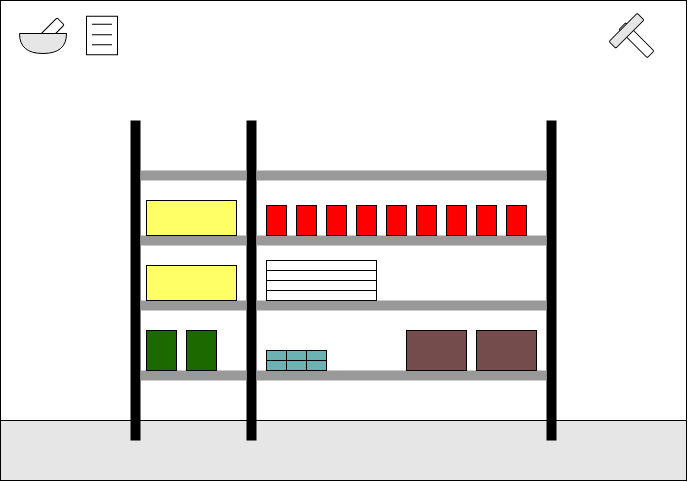
\includegraphics[width=\linewidth]{images/GUI-Skizze.png}
    \captionbelow{GUI im Normalzustand des Programms}
\end{figure}
\newpage
\begingroup
In dieser Skizze ist das Programm im Regal-Bearbeitungs-Modus. Der Hammer ist verschwunden, stattdessen gibt es einen Haken,
um die Bearbeitung abzuschließen. Die Zutaten werden gräulich dargestellt, die Stützen und Bretter hervorgehoben. Am oberen 
Bildschirmrand erscheint ein Reiter mit den Brett- und Stützenvorlagen.
\endgroup
\begin{figure}[h!]
    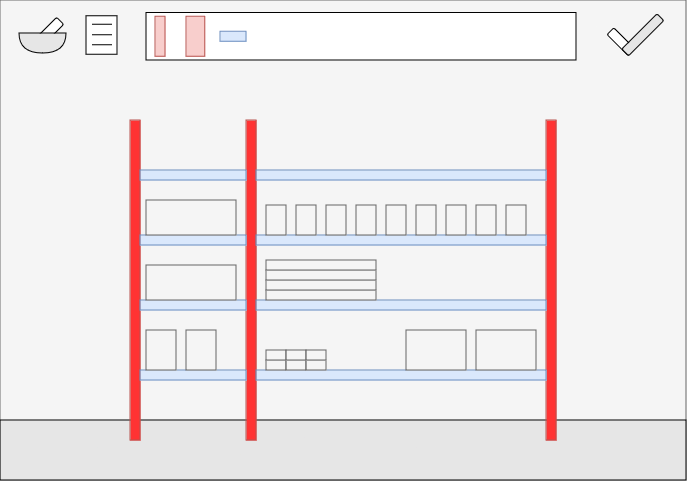
\includegraphics[width=\linewidth]{images/GUI-Skizze_Regal-Bearbeiten-Modus.drawio.png}
    \captionbelow{GUI im Regal-Bearbeitungs-Zustand}
\end{figure}
\newpage
\begingroup
In dieser Skizze ist das Programm im mitten in einer Bearbeitung. Ein paar Packungen wurden temporär aus dem Regal genommen
und sind nun ebenfalls im Reiter oben anzufinden. Währenddessen wird ein Brett mir einem separaten Kontext-Menü bearbeitet.
\endgroup
\begin{figure}[h!]
    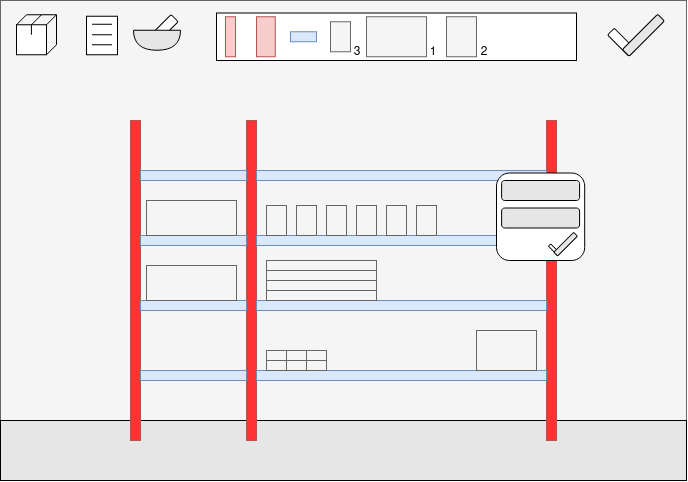
\includegraphics[width=\linewidth]{images/GUI-Skizze_Im-Bearbeiten.png}
    \captionbelow{GUI während eines Bearbeitungsvorgangs}
\end{figure}